\documentclass{article}
\usepackage{url}

\usepackage{tikz}
\usetikzlibrary{arrows.meta,calc,decorations.pathreplacing,shapes.geometric}
\tikzset{
    >=Stealth,
    er/.style={
        attr/.append style={align=center,draw,thick,ellipse,text width=2cm,text height=1.5ex,text depth=.25ex,font=\strut},
        entity/.append style={align=center,draw,thick,rectangle,text width=2cm,text height=2ex,text depth=.25ex,minimum height=1cm,font=\strut},
        rel/.append style={align=center,draw,thick,diamond,text width=2cm,text height=1.5ex,text depth=.25ex,font=\strut,fill=black!10,scale=0.65},
        isa/.append style={regular polygon, regular polygon sides=3,draw,thick,scale=0.65,font={ISA}},
        total/.append style={ultra thick},
        weak/.append style={ultra thick},
        once/.append style={->},
        strict/.append style={-Arc Barb[]},
        every edge/.append style={draw,thick}
    }
}

\usepackage[normalem]{ulem}
\newcommand{\key}[1]{\underline{\smash{#1}}}
\newcommand{\pkey}[1]{\dashuline{\smash{#1}}}


\begin{document}

\title{Examples of ER-Diagrams\\{\Large COMPSCI 2DB3: Databases--Winter 2023}}
\author{Jelle Hellings}
\date{{\normalsize
    Department of Computing and Software\\
    McMaster University
}}


\maketitle

\section{Other options}
\begin{itemize}
    \item There is a \verb!Tikz-er2! package for \LaTeX{} floating around.
    \item Software like yEd (\url{https://www.yworks.com/products/yed}) or Dia (\url{http://live.gnome.org/Dia}).
    \item The browser-based tools ERDPlus (\url{https://erdplus.com/}) and Diagrams.net (\url{https://app.diagrams.net/}, previously Draw.io).
    \item Microsoft Visio.
    \item Your favorite UML diagram draw program probably also has an option for ER-like diagrams.
    \item If all else fails: a (vector) drawing program.
\end{itemize}

\section{Figures from the slides}

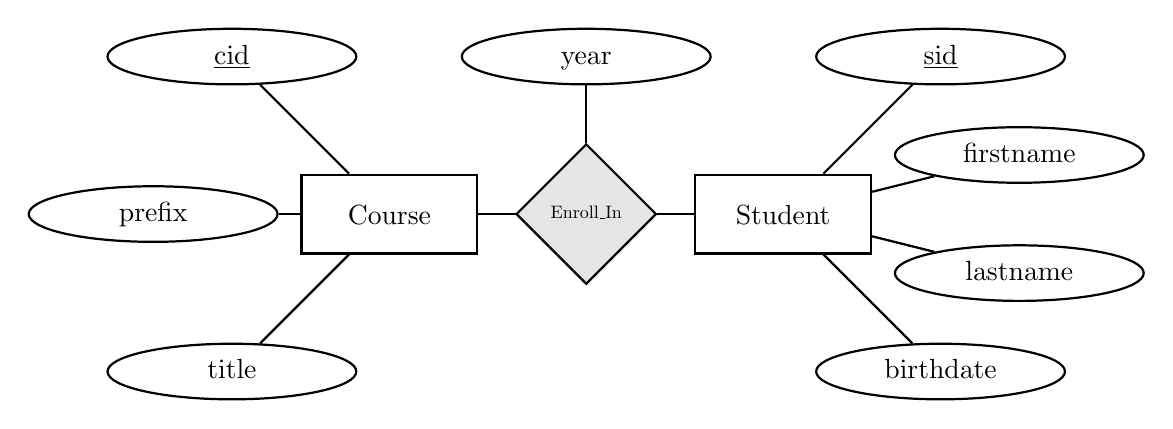
\begin{tikzpicture}[er]
    \node[entity] (s) at (0, 0) {Student};
    \node[attr] (sid) at (2, 2) {\key{sid}} edge[-] (s);
    \node[attr] (sage) at (2, -2) {birthdate} edge[-] (s);
        \node[attr] (sfname) at (3, 0.75) {firstname} edge[-] (s);
        \node[attr] (slname) at (3, -0.75) {lastname} edge[-] (s);
    \node[entity] (c) at (-5, 0) {Course};
    \node[attr] (cid) at (-7, 2) {\key{cid}} edge[-] (c);
    \node[attr] (cprefix) at (-8, 0) {prefix} edge[-] (c);
    \node[attr] (ctitle) at (-7, -2) {title} edge[-] (c);
    \node[rel] (r) at (-2.5, 0) {Enroll\_In} edge (c) edge (s);
    \node[attr] (ryear) at (-2.5, 2) {year} edge (r);
\end{tikzpicture}\\\bigskip

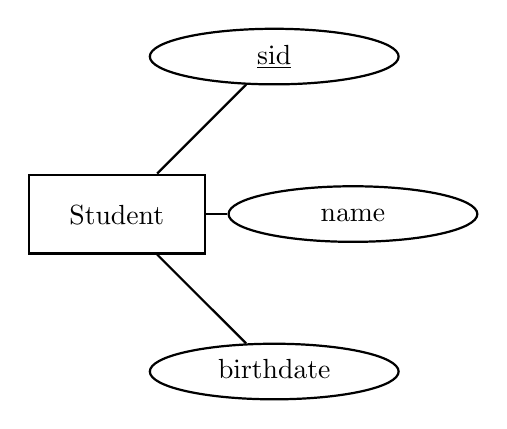
\begin{tikzpicture}[er]    
    \node[entity] (s) at (0, 0) {Student};
    \node[attr] (sid) at (2, 2) {\key{sid}} edge[-] (s);
    \node[attr] (sage) at (2, -2) {birthdate} edge[-] (s);
    \node[attr] (sfname) at (3, 0) {name} edge[-] (s);
\end{tikzpicture}\\\bigskip

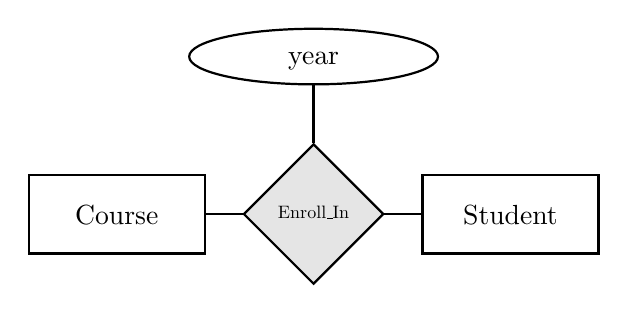
\begin{tikzpicture}[er]
    \node[entity] (s) at (0, 0) {Student};
    \node[entity] (c) at (-5, 0) {Course};
    \node[rel] (r) at (-2.5, 0) {Enroll\_In} edge (c) edge (s);
    \node[attr] (ryear) at (-2.5, 2) {year} edge (r);
\end{tikzpicture}\\\bigskip

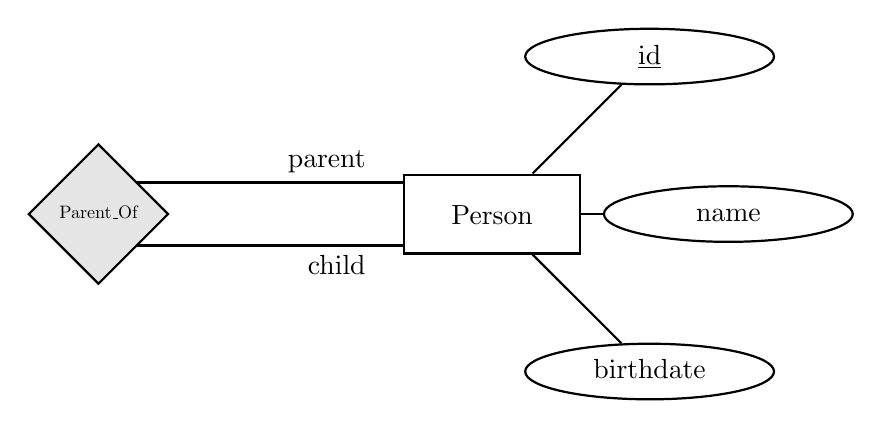
\begin{tikzpicture}[er]
    \node[entity] (s) at (0, 0) {Person};
    \node[attr] (sid) at (2, 2) {\key{id}} edge[-] (s);
    \node[attr] (sage) at (3, 0) {name} edge[-] (s);
    \node[attr] (sage) at (2, -2) {birthdate} edge[-] (s);

    \path (-5, 0.4) edge ($(s.west) + (0, 0.4)$)
          (-5, -0.4) edge ($(s.west) + (0, -0.4)$);
    \node[rel] (r) at (-5, 0) {Parent\_Of};

    \node[above left] at ($(s.west) + (-10pt, 0.4)$) {parent};
    \node[below left] at ($(s.west) + (-10pt, -0.4)$) {child};
\end{tikzpicture}\\\bigskip

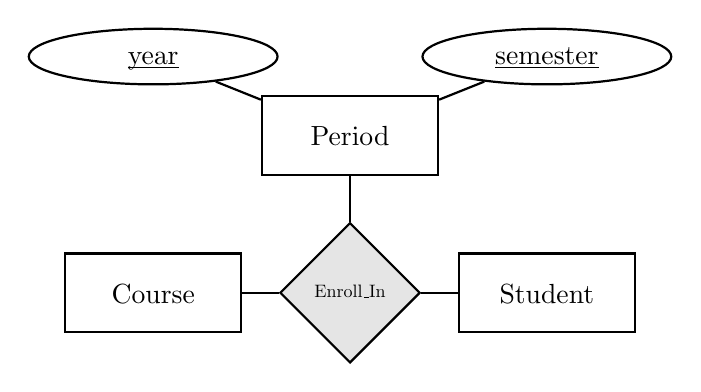
\begin{tikzpicture}[er]
    \node[entity] (s) at (0, 0) {Student};
    \node[entity] (c) at (-5, 0) {Course};
    \node[rel] (r) at (-2.5, 0) {Enroll\_In} edge (c) edge (s);
    \node[entity] (p) at (-2.5, 2) {Period} edge (r);
    \node[attr] (py) at (-5, 3) {\key{year}} edge[-] (p);
    \node[attr] (ps) at ( 0, 3) {\key{semester}} edge[-] (p);
\end{tikzpicture}\\\bigskip

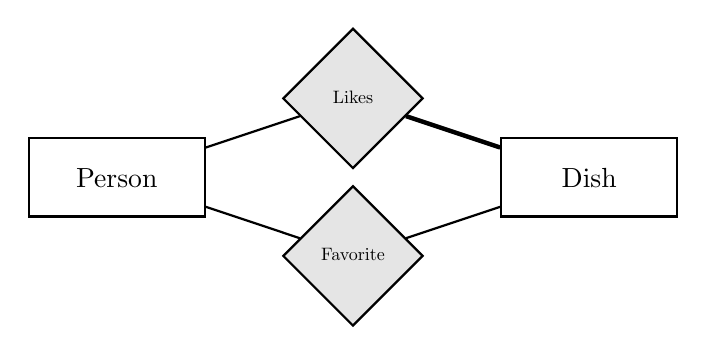
\begin{tikzpicture}[er]    
    \centering
    \node[entity] (p) at (0, 0) {Person};
    \node[entity] (d) at (6, 0) {Dish};

    \node[rel] (l) at (3, 1) {Likes} edge (p) edge (d);
    \node[rel] (f) at (3, -1) {Favorite};
    \path (f) edge (d);
    \path (p) edge (f);
    \path (l) edge[total] (d);
\end{tikzpicture}\\\bigskip

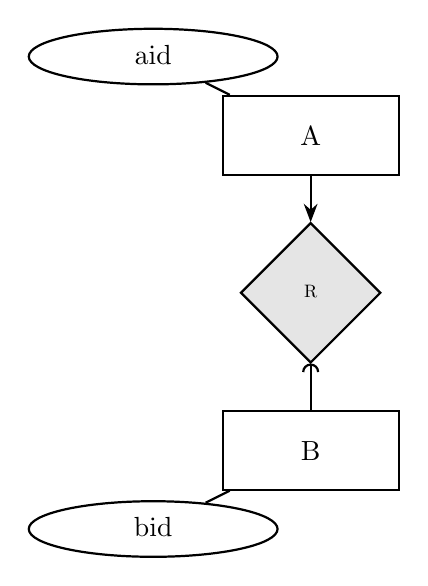
\begin{tikzpicture}[er]
    \node[entity] (a) at (0, 2) {A};
    \node[entity] (b) at (0, -2) {B};
    \node[attr] (aid) at (-2, 3) {aid} edge (a);
    \node[attr] (bid) at (-2, -3) {bid} edge (b);
    \node[rel] (r) at (0, 0) {R};
    \path (b) edge[strict] (r);
    \path (a) edge[once] (r);
\end{tikzpicture}\\\bigskip

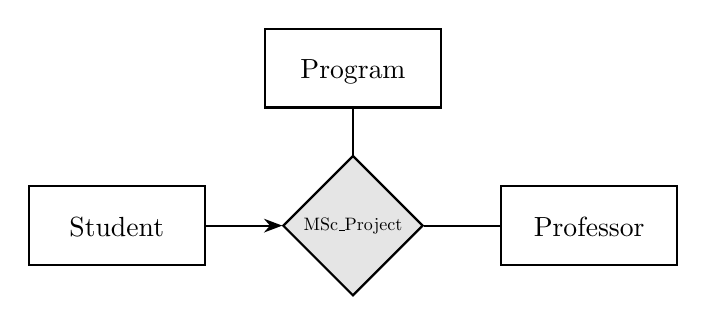
\begin{tikzpicture}[er]
    \node[entity] (s) at (-3, 0) {Student};
    \node[entity] (sv) at (3, 0) {Professor};
    \node[entity] (d) at (0, 2) {Program};
    \node[rel] (r) at (0, 0) {MSc\_Project};
    
    \path (r) edge (sv) edge (d);
    \path (s) edge[once] (r);
\end{tikzpicture}\\\bigskip

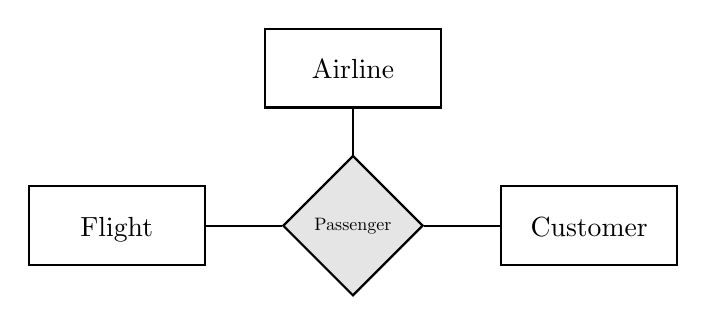
\begin{tikzpicture}[er]
    \node[entity] (f) at (-3, 0) {Flight};
    \node[entity] (c) at ( 3, 0) {Customer};
    \node[rel] (p) at (0, 0) {Passenger};
    \node[entity] (l) at (0, 2) {Airline};
    
    \path (p) edge (c) edge (f) edge (l);
\end{tikzpicture}\\\bigskip

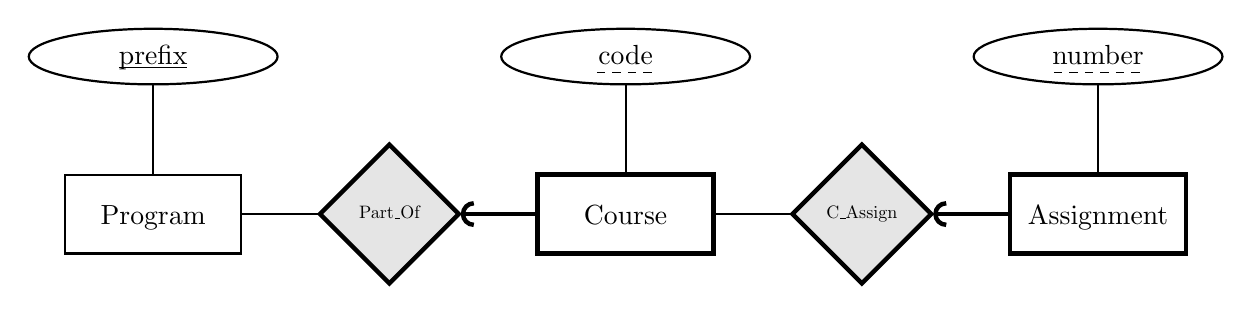
\begin{tikzpicture}[er]
    \node[entity] (prog) at (-6, 0) {Program};
    \node[attr] (ppre) at (-6, 2) {\key{prefix}} edge (prog);
    \node[rel,weak] (rweak) at (-3, 0) {Part\_Of} edge (prog);
    \node[entity,weak] (wcourse) at (0, 0) {Course} edge[strict,weak] (rweak);
    \node[attr] (wccode) at (0, 2) {\pkey{code}} edge (wcourse);

    \node[rel,weak] (cweak) at (3, 0) {C\_Assign} edge (wcourse);
    \node[entity,weak] (ass) at (6, 0) {Assignment} edge[strict,weak] (cweak);
    \node[attr] (asnum) at (6, 2) {\pkey{number}} edge (ass);
\end{tikzpicture}\\\bigskip

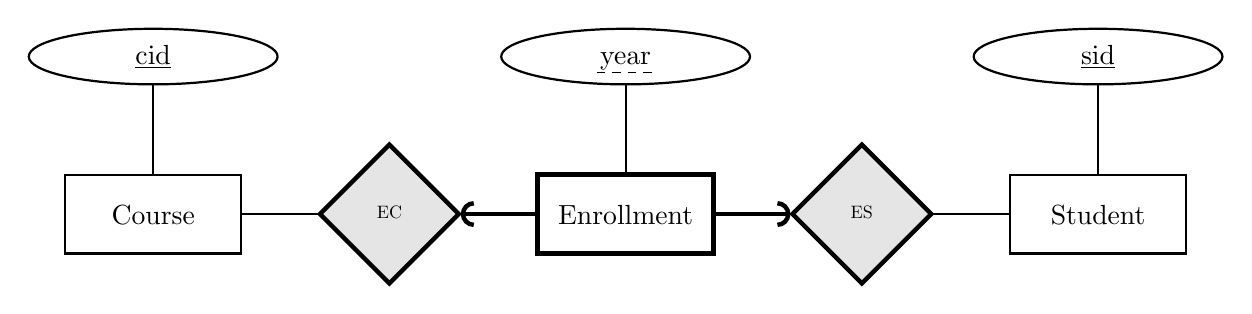
\begin{tikzpicture}[er]
    \node[entity] (s) at (6, 0) {Student};
    \node[attr] (sid) at (6, 2) {\key{sid}} edge[-] (s);
    \node[entity] (c) at (-6, 0) {Course};
    \node[attr] (cid) at (-6, 2) {\key{cid}} edge[-] (c);
    \node[rel,weak] (es) at ( 3, 0) {ES} edge (s);
    \node[rel,weak] (ec) at (-3, 0) {EC} edge (c);
    \node[entity,weak] (ei) at (0, 0) {Enrollment} edge[strict,weak] (es) edge[strict,weak] (ec);
    \node[attr] at (0, 2) {\pkey{year}} edge (ei);
\end{tikzpicture}\\\bigskip

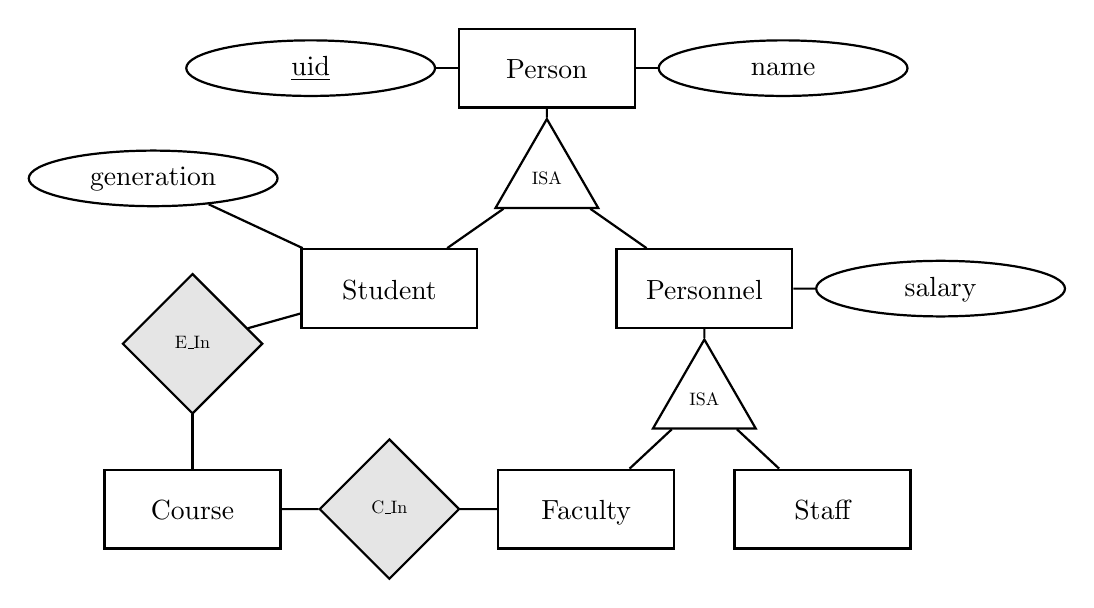
\begin{tikzpicture}[er,yscale=0.7]
    \node[entity] (p) at (0, 0) {Person};
    \node[attr] (pid) at (-3, 0) {\key{uid}} edge (p);
    \node[attr] (pname) at (3, 0) {name} edge (p);

    \node[isa] (isa1) at (0, -2) {} edge (p);

    \node[entity] (s) at (-2, -4) {Student} edge (isa1);
    \node[attr] (sgen) at (-5, -2) {generation} edge (s);
    \node[entity] (pers) at (2, -4) {Personnel} edge (isa1);
    \node[attr] (sgen) at (5, -4) {salary} edge (pers);
    \node[isa] (isa2) at (2, -6) {} edge (pers);

    \node[entity] (pf) at (0.5, -8) {Faculty} edge (isa2);
    \node[entity] (ps) at (3.5, -8) {Staff} edge (isa2);
    \node[entity] (c) at (-4.5, -8) {Course};
    \node[rel] (cin) at (-2, -8) {C\_In} edge (c) edge (pf);
    \node[rel] (ein) at (-4.5, -5) {E\_In} edge (c) edge (s);
\end{tikzpicture}\\\bigskip

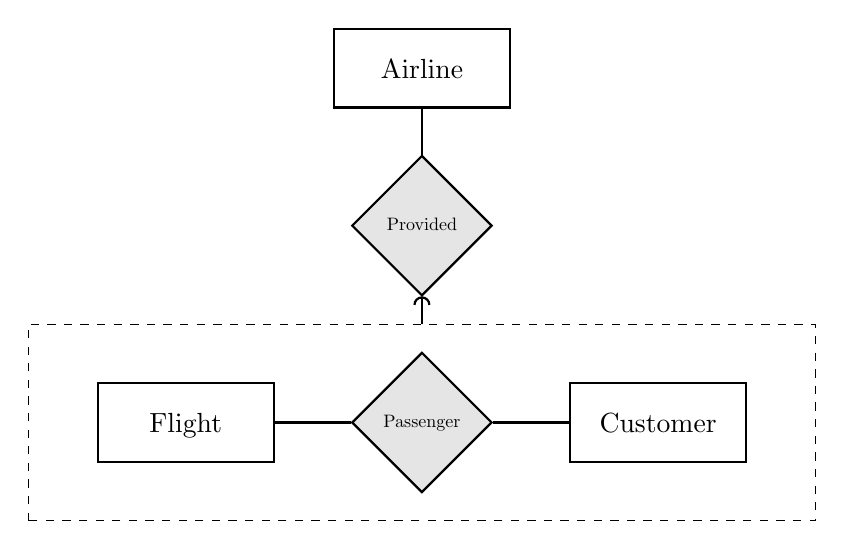
\begin{tikzpicture}[er]
    \draw[dashed] (-5, -1.25) rectangle (5, 1.25);
    \node[entity] (l) at (0, 4.5) {Airline};
    
        \node[entity] (f) at (-3, 0) {Flight};
        \node[entity] (c) at ( 3, 0) {Customer};
        \node[rel] (p) at (0, 0) {Passenger};
        \path (p) edge (c) edge (f);
        \node[rel] (r) at (0, 2.5) {Provided};
        \path (l) edge (r);
        \path (0, 1.25) edge[strict] (r);
\end{tikzpicture}\\\bigskip


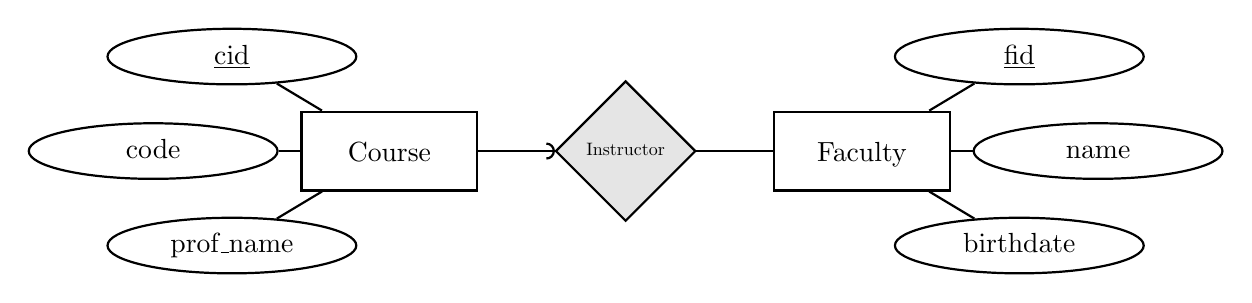
\begin{tikzpicture}[er,yscale=0.6]
    \node[entity] (f) at (3, 0) {Faculty};
    \node[attr] (fid) at (5, 2) {\key{fid}} edge (f);
    \node[attr] (fname) at (6, 0) {name} edge (f);
    \node[attr] (fbday) at (5, -2) {birthdate} edge (f);

    \node[rel] (i) at (0, 0) {Instructor} edge (f);

    \node[entity] (c) at (-3, 0) {Course} edge[strict] (i);
    \node[attr] (cid) at (-5, 2) {\key{cid}} edge[-] (c);
    \node[attr] (ccode) at (-6, 0) {code} edge[-] (c);
    \node[attr] (cpname) at (-5, -2) {prof\_name} edge[-] (c);
\end{tikzpicture}\\\bigskip

\end{document}